%-------------------------------------------------------------------------------------------------
\subsection{MEX 3-3: Inverse Analysis of Reiche Zeche Field Data}

Data management for model used throughout MEX 3-3 (see \ref{sec:mex09}).

Link to the data set stored at the Gitlab server located at the Institute of Applied Mechanics, University of Stuttgart:\\
\hyperlink{https://galilei.isr.uni-stuttgart.de/gitlab/schmidt/geomint}{https://galilei.isr.uni-stuttgart.de/gitlab/schmidt/geomint}\\
\begin{figure}[!ht]
\begin{center}
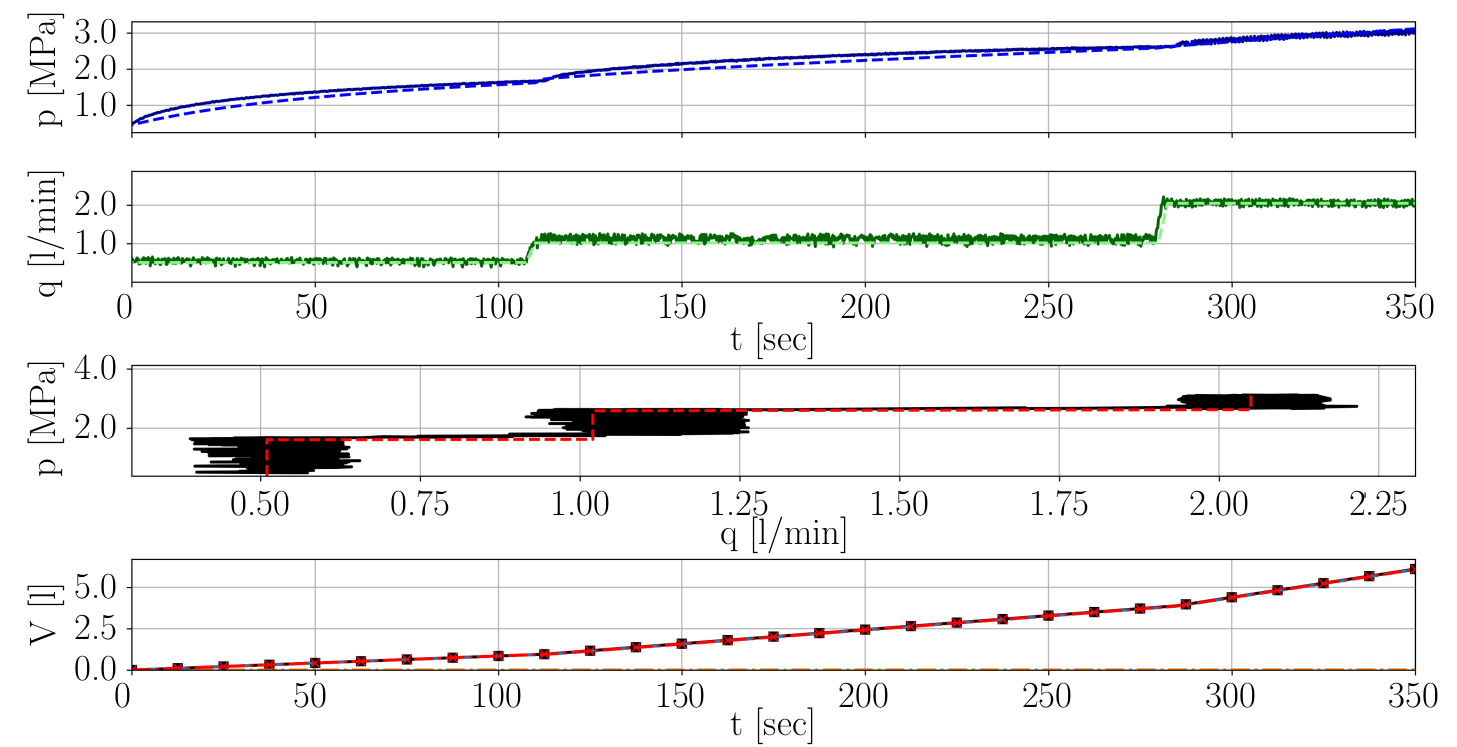
\includegraphics[width=1.0\textwidth]{./figures/data_management_reiche_zeche_40_6.png}
\end{center}
\caption{Visualisation of data obtained from the pre-compiled executable used for inverse analysis computations of pumping tests performed at Reiche Zeche at a depth of $40.6\,$m.}
\label{fig:DataReicheZeche}
\end{figure}

The uploaded data set contains two compiled executables for simulations to fit experimental data for the Reiche Zeche fracture characterization tests and to reproduce the non-linear response throughout harmonic testing of a single fracture on the laboratory scale like described in section \ref{sec:mex09}. The folder includes executables, input files and the used discretization in terms of meshing files, required to perform the simulations. README.txt files provide further informations how to start the simulations.

\begin{table}[!ht]
\caption{MEX 3-3: Reiche Zeche Data}
\label{tab:dms-mex3-3}
\small
\begin{tabular}{R{3cm}|L{7cm}}
\hline
%
Data label & GeomInt | UoS | Data Set Reiche Zeche \\
URI &  https://galilei.isr.uni-stuttgart.de/gitlab/schmidt/geomint\\
Subject  &  Non-linear hydro-mechanics / fracture flow\\
Type of data  &  executable, mesh input, parameter input\\
Dataquality  &  quality assured data \\
Status of data  &  unprocessed data\\
Dataformat  & txt, msh, linux executable\\
Creators  &  University of Stuttgart, Institute of Applied Mechancis - Continuum Mechanics, Pfaffenwaldring 7, 70569 Stuttgart\\
Source/Origin & In-house code \\
Publisher  &  University of Stuttgart, Institute of Applied Mechancis - Continuum Mechanics, Pfaffenwaldring 7, 70569 Stuttgart \\
Rights holders & University of Stuttgart, Institute of Applied Mechancis - Continuum Mechanics, Pfaffenwaldring 7, 70569 Stuttgart \\
Contributors &  University of Stuttgart, Institute of Applied Mechancis - Continuum Mechanics, Patrick Schmidt and Holger Steeb\\
Time or Period of creation &  2018-2019\\
Language of the content &  English\\
Update policy &  stored data is final\\
Access permissions &  full access\\
%
\hline
\end{tabular}
\end{table}